\chapter{Background}\section{An Overview about image processing}
Nowadays, we have a lot of programs which used to edit photos (e.g. Photoshop, Gimp, MSPaint,...). By applying some techniques, we can effect some properties to change the images such as: scaling, blurring, rotating image,etc. Actually, an image is presented by a set of pixels. Each pixel carries a value which presents the color at that location. When combing the values of all the pixels, we obtain the image as it in the real word. The changing on image really changes the value of each pixel in an image. Behind the techniques in these programs are mathematical operations and a field that used mathematical operation to an input image,  which is \textit{image processing}. The output of the image processing process may be either an image or a set of characteristics related to the image. And most of the image processing techniques are performed on two-dimensional images. In image processing, we have a lot of operators. In this chapter, we introduce some basis operations that are often used as the object of this internship.
\section{Image filtering}
Image filtering is a process to modify or enhance the image's quality. This is known as a ``neighborhood" operation. The neighborhood is a set of pixels around a selected pixel. In image processing, with a pixel, we may obtain have 4-neighbors or 8-neighbors of it. Image filtering determines the value at the selected pixel by applying some operations with the values of its neighbors. One of the filtering operators is smoothing, also named blurring. This technique is used in preprocessing steps, particularly in noise reduction. With a matrix called kernel. It was sliding over the image. At each position, the output of a value at that position is calculated by meaning its neighborhoods value.
In image processing, we have many filtering techniques. But there are 2 main types:\\[0.2cm]
\textbf{Linear filter}: The idea behind this filtering method is replacing the value of every pixel in the image by the average of the gray levels in the neighborhood defined by the filter mask. By this work, this filter sometime are called averaging filter. The result of this process is an image with the sharp edges reduced in gray level, it also reduces the noise because the noise is typically and random in the image. The mask is a matrix and its useful for blurring, sharpening, edge-detection, etc. The output image is accomplished by convoluting between a mask and an image.\\[0.2cm]
\textbf{Order-Statistics filter}: By ordering the pixels in the image and then replacing the values of the center pixel with the value determined by the ranking result. Median filter is an example of this technique.
\section{Histogram}
Histogram is a representation of the distribution of data on the regions (we called bins) in the data range. The bins are the number of sub-ranges when we divide the entire data range into several small intervals (i.e. With the range of [0 - 255] and the size of each sub-range (bin) is 16, the number of bins is $256/16 = 16$ bins. The first bin range is [0 - 15], the second range is {15 - 30}, and so on). The value at each bin is the number of data which have value belong to it. Normally, histogram is representing by the columns chart with x-axis represent as for the number of bins, and y-axis represent as for the value of each bin.\\
Histogram can be used effectively for image enhancement, it's also useful in many image processing applications, such as image compression and segmentation.\\[0.3cm]
\begin{figure}[h!]
\centering
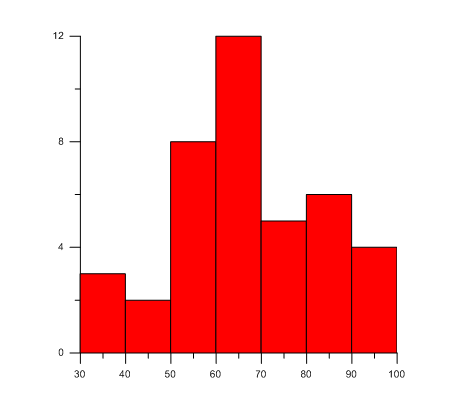
\includegraphics[scale=2]{images/histogram}
\caption{An example about histogram}
\label{fig:figure_31}
\end{figure}
\textbf{Histogram equation}: is a method that allows adjusting the contrast using the histogram of image. It maps the distribution on a histogram to a wider distribution of the intensity values. By applying this, the image could be brighter.\\[0.2cm]
\textbf{Histogram matching}: is the method that adjusts two images using the histogram. This method is finished by calculating the cumulative distribution functions of the two histograms to finding the histogram matching function. Finally, applying the matching function on each pixel of the image to get the result.
\section{Segmentation}
Segmentation subdivides an image into the regions. The size of the regions is depended on the problem being solved. This mean, segmentation should stop when the regions of interest in application have been detected. In real world, the segmentation is applied to many fields such as machine vision, medical imaging, object detection, etc. The most what of segmentation algorithms are based on the basic properties of intensity values: discontinuity and similarity. In the first case, the segmentation based on abrupt changes in intensity. In the second case, the image segmentation based on a predefined criteria. It means the image was segmented into regions those are similar according to a set of criterias. And, we have many the methods to segment an image such as thresholding method, region growing method, clustering method, histogram-based method, etc.\\[0.2 cm]
\textbf{Thresholding} is the simplest method of image segmentation. Thresholding uses a particular threshold value ``t", which splits the image into two parts: the first part includes pixels which have the value greater than ``t", and the second part contains the pixels smaller than ``t". With this technique, thresholding can be used to create an binary image from a gray scale image. In fact, we have many type of thresholds, as follows:
\begin{itemize}
\item \textit{Global thresholding}, when \textit{t} is a constant over an entire image
\item \textit{Variable thresholding}, when \textit{t} changes over an image
\item \textit{Local or regional thresholding}, is variable threshoding in a region of an image
\item \textit{Dynamic or adaptive thresholding}, if \textit{t} depends on the spatial coordinates.
\item \textit{Multiple thresholding}, thresholding on 3 dominant modes (color image)
\end{itemize}
\textbf{Canny} algorithm is an edge detection algorithm that uses to detect the structure of an image. The process of this algorithm can be broken into the steps as follows \footnote{https://en.wikipedia.org/wiki/Canny\_edge\_detector}:
\begin{itemize}
\item Apply the Gaussian filter to smooth the image (remove the noise),
\item Find the intensity gradients of the image,
\item Apply non-maximum suppression to get rid of spurious response to edge detection,
\item Apply double threshold to determine potential edges,
\item Track edges.
\end{itemize}
\section{Color processing$^{\cite{oscarbook}}$}\label{color_model}
The usage of colors in image processing are not limit in identifying or extracting an object from its scene, it also a factor of image analysis. Color processing can be a effected on each component image individually or works directly with pixels-based on a color model. The color models is a specification of colors in some standard, generally accept way such as BGR, CMY, HSV or Grayscale model.
\begin{itemize}
\item BGR model: using blue, green, red as three primary colors. Image presented in this model consists of three components images for each primary color.
\item CMY model: used for hardcopy devices. Based on the BGR mode, each value in CMY mode was computed by integrating the 2 primary colors in BGR. Specific, C (cyan) is consist of green and blue, M (magenta) is consist of red and blue and Y (yellow) is consist of red and green.
\item HSV model: different from BGR, HSV uses the 3 components which are hue, saturation and brightness to represent image. Hue is a color attribute which describes the pure color (yellow, orange, red) and saturation gives a degree to pick the pure color diluted by white light. Brightness is a notation of intensity for color sensation.
\item Grayscale model: The colors in grayscale are black and white because it just carry the intensity information on each pixel. Because that, the image in grayscale mode was called black and white image. The color of each pixels in image from black, where have weakest intensity to white at the strongest intensity.
\end{itemize}
The most popular color operations in image processing fields is transformation. It is a process to convert image between the color models by using a transform expression such as BGR to HSV, HSV to BGR, BGR to Grayscale.\\[0.2cm]
Besides, by considering a specific characteristic of each color space, allow as us classify the pixels in the image. This idea can be used to segment objects of an image. HSV model is widely used to compare the color because the range of color (Hue value) is specific.
\begin{figure}[h!]
\centering
\subfloat[An image in BGR mode (source image)]{\label{fig:example_1}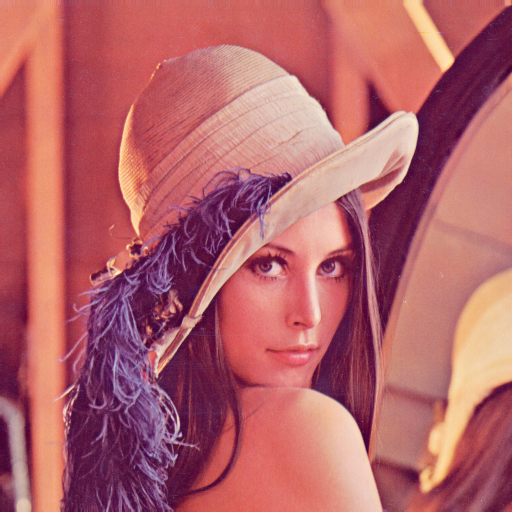
\includegraphics[width=0.4\textwidth]{./images/lenna}}~~
\subfloat[An image in Gray mode]{\label{fig:example_2}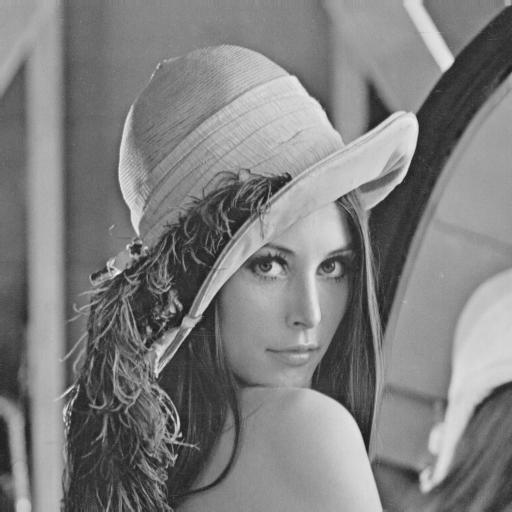
\includegraphics[width=0.4\textwidth]{./images/lenna_gray}}
\caption{The images with color transformation from BGR to Gray}
\label{fig:figure_31}
\end{figure}

